\documentclass[conference]{IEEEtran}
\usepackage[T1]{fontenc}
\usepackage{amsmath,amssymb}
\usepackage{graphicx}
\usepackage{booktabs}
\usepackage{multirow}
\usepackage{array}
\usepackage{xcolor}
\usepackage{algorithm}
\usepackage[noend]{algpseudocode}
\usepackage{tikz}
\usetikzlibrary{arrows.meta,positioning,calc}
\usepackage{cite}
\usepackage{url}
\usepackage[hidelinks]{hyperref}
\graphicspath{{figures/}}

\newcommand{\dc}{$\Delta$Context}
\newcommand{\dcr}{$\Delta$Context-R}
\newcommand{\todo}[1]{\textcolor{red}{[#1]}}
\renewcommand{\algorithmicrequire}{\textbf{Input:}}
\renewcommand{\algorithmicensure}{\textbf{Output:}}

\begin{document}

\title{\dcr{}: Budget-Aware Retrieval over an Online Topic Store for Long-Term Conversational Memory}

\author{\IEEEauthorblockN{Pravin Raj}
\IEEEauthorblockA{\todo{Department, Institution}\\
\todo{City, Country}\\
\todo{e-mail}}
\and
\IEEEauthorblockN{\todo{Co-author / supervisor}}
\IEEEauthorblockA{\todo{Department, Institution}\\
\todo{City, Country}\\
\todo{e-mail}}}

\maketitle

\begin{abstract}
Long-term chat assistants must answer from histories far longer than their
context window. Recent segment-level memory stores a conversation as topical
segments, denoises them by prompt compression and retrieves whole segments, but
it needs a large-model call per session to segment, and whole segments exhaust
small context budgets. This paper proposes \dcr{}. The history is stored as
topics by an online delayed-commitment segmenter that needs no language model
and never revises a boundary. Retrieval ranks turns by fusing lexical, dense
and topic evidence, then spends the budget on the user's own statements inside
the most relevant topics. On LongMemEval-S, with one 2,048-token budget and one
3B reader, \dcr{} raises evidence recall from 0.64 to 0.91 and answer F1 from
0.270 to 0.369 over segment-level memory, and at 4,096 tokens it beats strong
turn-level hybrid retrieval (recall 0.969 vs.\ 0.912). Controlled ablations show
that budget-aware reading of user turns drives the gain.
\end{abstract}

\begin{IEEEkeywords}
Conversational memory, retrieval-augmented generation, topic segmentation,
context budget, large language models, long-term dialogue.
\end{IEEEkeywords}

% =====================================================================
\section{Introduction}

\IEEEPARstart{D}{ialogue} systems built on large language models (LLMs) are
becoming long-lived assistants \cite{ni2023survey,wang2024agents}, and an
assistant that remembers earlier sessions needs a memory that grows without
bound \cite{zhang2025memory}. Placing the whole history in the prompt is not an
answer: attention cost grows with input length \cite{tay2022efficient}, models
use the middle of long inputs unreliably \cite{liu2024lost}, and missing or
irrelevant context causes hallucination \cite{huang2025hallucination}. Practical
systems therefore retrieve, for each question, a few past passages under a token
budget \cite{wu2026rag,zhao2024dense,pan2024vectordb}, summarise old turns
\cite{wang2025recursive}, or manage memory with update and paging rules
\cite{zhong2024memorybank,packer2023memgpt}.

How the history is cut into memory units matters. LongMemEval showed that
long-context LLMs lose about 30\% accuracy on chat histories of $\sim$115K tokens
and that the granularity of stored values is a key design choice
\cite{wu2025longmemeval}. SeCom \cite{pan2025secom} went further: it segments
every session into topics with an LLM, denoises each segment with LLMLingua-2
prompt compression \cite{pan2024llmlingua2}, and retrieves whole segments,
outperforming turn-level and session-level memory on two benchmarks. Topic
structure is also known to help dialogue understanding
\cite{ma2024topicaware,xu2025umlf}, and chunking choices change retrieval
quality \cite{lavarec2026chunking}.

\textbf{Problem statement.} Segment-level memory has two costs. Building it
takes one LLM call per session, and retrieving whole segments spends a small
budget on a few long units, much of them assistant text. The question is how
to store a growing chat as topics without an LLM, and how to retrieve from that
store so that a fixed budget carries the most evidence.

\textbf{Objective.} To build a topic-indexed conversational memory with no LLM
in the loop, and a retrieval rule that beats segment-level memory and strong
turn-level retrieval at the same token budget and reader.

\textbf{Contributions.}
\begin{enumerate}
\item \dcr{}, a budget-aware retrieval method over an online topic store. It
fuses BM25, dense and topic ranks, reads the user's turns inside the most
relevant topics, and reserves part of the budget for them.
\item A controlled re-implementation of SeCom and of turn-, exchange- and
session-level memory, with every unit, key (raw or LLMLingua-2) and retriever
evaluated under one budget, one reader and dev-only tuning.
\item On LongMemEval-S, \dcr{} improves on SeCom by 0.27 evidence recall and
0.099 answer F1 (a 37\% relative gain) and beats turn-level hybrid retrieval at
4,096 tokens, without any LLM call to build the memory.
\item An ablation showing what drives the gain: reading short user turns within
the budget, not topic structure as such. The online topics match true sessions
and beat fixed chunks, but topic-free budget rules perform equally well.
\end{enumerate}

\textbf{Organisation.} Section~\ref{sec:lit} reviews related work,
Section~\ref{sec:method} presents \dcr{}, Section~\ref{sec:results} reports
results, Section~\ref{sec:comp} compares with existing works, and
Section~\ref{sec:concl} concludes.

% =====================================================================
\section{Literature Review}
\label{sec:lit}

\textbf{Memory systems.} MemoryBank \cite{zhong2024memorybank} stores memories
with summaries and a forgetting rule; MemGPT \cite{packer2023memgpt} lets the
LLM page information between prompt and storage; recursive summarisation
\cite{wang2025recursive} rewrites a running memory; LongMemEval
\cite{wu2025longmemeval} decomposes sessions into rounds and expands keys with
LLM-extracted facts. SeCom \cite{pan2025secom} is the closest work: segment-level
units, compression-based denoising with LLMLingua-2 \cite{pan2024llmlingua2},
and BM25 or MPNet retrieval.

\textbf{Topic segmentation.} TextTiling \cite{hearst1997texttiling} cuts at
depth minima of a similarity curve and is the decoder of neural methods such as
CSM \cite{xing2021csm}; DialSTART \cite{gao2023dialstart} and UMLF
\cite{xu2025umlf} learn topic-aware representations, and SuperDialseg
\cite{jiang2023superdialseg} supplies supervised data. All segment complete
dialogues offline. Semantic chunking \cite{langchain2024semantic} and the
chunkers compared by Lavarec and Du \cite{lavarec2026chunking} also need the
whole text.

\textbf{Retrieval.} BM25 \cite{robertson2009bm25} and dense sentence encoders
\cite{reimers2019sbert,song2020mpnet} are the standard retrievers, and
reciprocal-rank fusion (RRF) \cite{cormack2009rrf} combines them without
calibration. Label-free semantic structure has also proven useful for named
entities \cite{veena2023agroner}, relation extraction for knowledge graphs
\cite{veena2023relation}, aspect extraction with BERT-guided topic models
\cite{venugopalan2022guidedlda} and topic-guided summarisation
\cite{gurusamy2023summarization}. Table~\ref{tab:lit} summarises ten recent
works.

\begin{table*}[t]
\centering
\caption{Ten recent related works and their drawback for a budget-limited conversational memory.}
\label{tab:lit}
\footnotesize
\setlength{\tabcolsep}{4pt}
\renewcommand{\arraystretch}{1.08}
\begin{tabular}{@{}p{2.6cm}p{0.6cm}p{4.4cm}p{3.7cm}p{5.2cm}@{}}
\toprule
Work & Year & Algorithm & Advantage & Drawback for our setting \\
\midrule
MemoryBank \cite{zhong2024memorybank} & 2024 & Memory store, summaries, forgetting curve, dense retrieval & Persistent, user-adaptive & Flat units; no budget-aware selection \\
MemGPT \cite{packer2023memgpt} & 2023 & LLM-managed paging between prompt and storage & Unbounded virtual context & An LLM call per memory operation \\
Recursive summaries \cite{wang2025recursive} & 2025 & LLM rewrites memory from old memory and new turns & Compact memory & Lossy; verbatim evidence is lost \\
LongMemEval \cite{wu2025longmemeval} & 2025 & Round-level values, fact-augmented keys, time-aware queries & Systematic memory study & Key expansion needs an LLM per round \\
SeCom \cite{pan2025secom} & 2025 & LLM segmentation, LLMLingua-2 denoising, segment retrieval & Beats turn and session memory & LLM call per session; whole segments fill small budgets \\
LLMLingua-2 \cite{pan2024llmlingua2} & 2024 & Token classification keeps informative tokens & Fast, faithful compression & A 560M-parameter model over all stored text \\
UMLF \cite{xu2025umlf} & 2025 & Joint discourse parsing and topic segmentation & Best unsupervised segmentation & Offline; several large encoders \\
DialSTART \cite{gao2023dialstart} & 2023 & Topic-aware contrastive utterance learning & Strong unsupervised accuracy & Needs in-domain training; offline \\
Topic-aware comprehension \cite{ma2024topicaware} & 2024 & Unsupervised topic blocks + dual-attention matching & Topics aid response selection & Segments finished passages; no retrieval budget \\
Chunking for RAG \cite{lavarec2026chunking} & 2026 & Fixed, recursive, semantic, LLM chunking compared & Chunking changes RAG quality & Documents with structure that chats lack \\
\bottomrule
\end{tabular}
\end{table*}

\textbf{Identified problem.} Existing memories either retrieve fixed units that
ignore the budget, or build topic units with an LLM and retrieve them whole. No
prior work builds topics online without an LLM and decides, within a token
budget, which turns of which topics to read, or tests what actually makes such
retrieval work.

% =====================================================================
\section{Proposed Work}
\label{sec:method}

\dcr{} has two stages and four phases (Fig.~\ref{fig:arch}). Storage (Phases
1--3) runs once per incoming turn; retrieval (Phase 4) runs once per question.

\begin{figure*}[t]
\centering
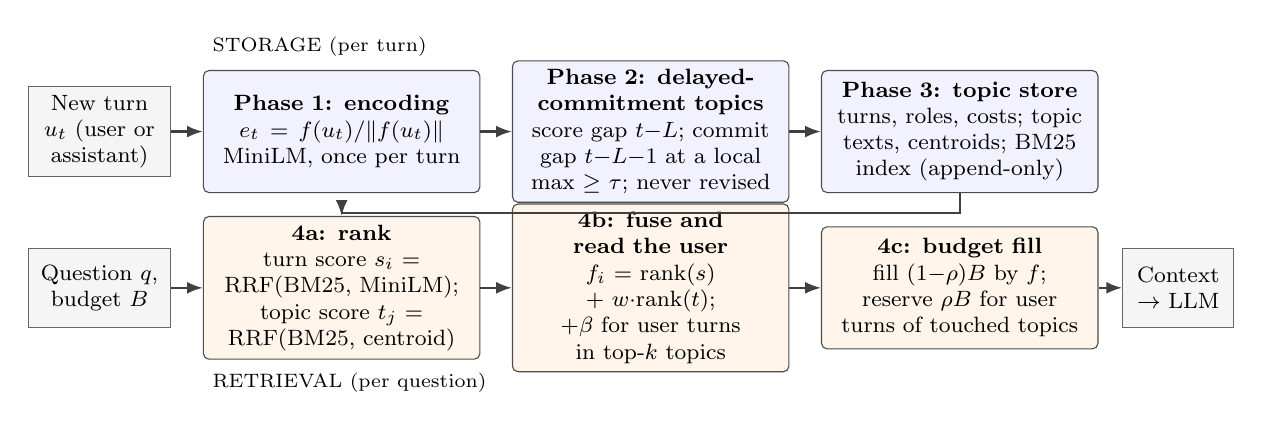
\begin{tikzpicture}[
  node distance=4mm,
  box/.style={draw=black!70, rounded corners=2pt, fill=blue!5, align=center, text width=3.3cm,
              minimum height=1.55cm, font=\footnotesize, inner sep=3pt},
  rbox/.style={box, fill=orange!8},
  io/.style={draw=black!60, fill=black!4, align=center, text width=1.6cm, minimum height=1.0cm,
             font=\footnotesize, inner sep=3pt},
  arr/.style={-{Latex[length=2mm]}, thick, black!75},
  lab/.style={font=\footnotesize\bfseries, anchor=west}]
\node[io] (in) {New turn $u_t$ (user or assistant)};
\node[box, right=of in] (p1) {\textbf{Phase 1: encoding}\\$e_t=f(u_t)/\lVert f(u_t)\rVert$\\MiniLM, once per turn};
\node[box, right=of p1] (p2) {\textbf{Phase 2: delayed-commitment topics}\\score gap $t{-}L$; commit gap $t{-}L{-}1$ at a local max $\ge\tau$; never revised};
\node[box, right=of p2] (p3) {\textbf{Phase 3: topic store}\\turns, roles, costs; topic texts, centroids; BM25 index (append-only)};
\node[io, below=9mm of in] (q) {Question $q$, budget $B$};
\node[rbox, right=of q] (p4a) {\textbf{4a: rank}\\turn score $s_i$ = RRF(BM25, MiniLM);\\topic score $t_j$ = RRF(BM25, centroid)};
\node[rbox, right=of p4a] (p4b) {\textbf{4b: fuse and read the user}\\$f_i$ = rank($s$) + $w\cdot$rank($t$);\\+$\beta$ for user turns in top-$k$ topics};
\node[rbox, right=of p4b] (p4c) {\textbf{4c: budget fill}\\fill $(1{-}\rho)B$ by $f$; reserve $\rho B$ for user turns of touched topics};
\node[io, right=3mm of p4c, text width=1.2cm] (out) {Context $\rightarrow$ LLM};
\draw[arr] (in) -- (p1); \draw[arr] (p1) -- (p2); \draw[arr] (p2) -- (p3);
\draw[arr] (q) -- (p4a); \draw[arr] (p4a) -- (p4b); \draw[arr] (p4b) -- (p4c); \draw[arr] (p4c) -- (out);
\draw[arr] (p3.south) -- ++(0,-0.25) -| (p4a.north);
\node[font=\scriptsize, above=0.5mm of p1.north west, anchor=south west] {STORAGE (per turn)};
\node[font=\scriptsize, below=0.5mm of p4a.south west, anchor=north west] {RETRIEVAL (per question)};
\end{tikzpicture}
\caption{\dcr{}. Storage builds a topic store online with no language model;
retrieval ranks turns with lexical, dense and topic evidence and spends the
budget on the user's statements inside the most relevant topics.}
\label{fig:arch}
\end{figure*}

\subsection{Phases 1--3: online topic storage}
Each turn is prefixed with its role and encoded once by a sentence encoder $f$
(all-MiniLM-L6-v2 \cite{reimers2019sbert}). Topics are found by \dc{}'s
delayed-commitment detector. With $\mu(i,j)$ the normalised mean of
$e_i,\dots,e_j$ and $a$ the start of the open topic, gap $g$ (between turns $g$
and $g{+}1$) is scored once $L$ further turns exist:
\begin{equation}
s_g = 1-\mu\bigl(\max(a,g-c+1),\,g\bigr)^{\top}\mu\bigl(g+1,\,g+L\bigr).
\end{equation}
Gap $g$ is decided one turn later and becomes a boundary only if
$s_g\ge s_{g-1}$, $s_g\ge s_{g+1}$ and $s_g\ge\tau$; a committed boundary is
never revised, so the store is append-only. We use the setting tuned on
LongMemEval dev histories for segmentation accuracy ($L{=}3$, $c{=}3$,
$\tau{=}0.75$), fixed before any retrieval experiment. Each topic keeps
its turns, the role and token cost of every turn, its text for BM25, and its
centroid. No LLM is called at any point.

\subsection{Phase 4: budget-aware topic retrieval}
Algorithm~\ref{alg:ret} gives the procedure. For a question $q$, each turn $i$
receives a hybrid score $s_i$, the RRF \cite{cormack2009rrf} of its BM25 rank
\cite{robertson2009bm25} and its MiniLM cosine rank; each topic $j$ receives
$t_j$, the RRF of the BM25 rank of its text and the cosine rank of its centroid.
With $r(\cdot)$ the rank (0 = best) and $K{=}60$, the fused score is
\begin{align}
f_i={}&\frac{1}{K+1+r(s)_i}+\frac{w}{K+1+r(t)_{\tau(i)}}\nonumber\\
&+\frac{\beta}{K+1}\,\mathbf{1}\bigl[\mathrm{user}(i)\wedge r(t)_{\tau(i)}<k\bigr],
\label{eq:fused}
\end{align}
where $\tau(i)$ is the topic of turn $i$. The first term ranks turns, the second
prefers turns in relevant topics, and the third reads what the user said in the
$k$ most relevant topics. Turns are packed greedily by $f$ into $(1-\rho)B$
tokens; the reserved $\rho B$ then takes the remaining user turns of every topic
already read from, and any leftover budget takes other turns by $f$. The context
is shown in chronological order with session dates.

\textbf{Why read the user.} In a personal-assistant memory the facts asked about
are mostly what the user said, and user turns are short while assistant replies
are long. A ranking that ignores cost spends the budget on a few long replies.
Section~\ref{sec:comp} shows that two thirds of the evidence a turn ranker misses
lies inside topics it already read from, which is what the reserve recovers.

\textbf{Parameters and cost.} $w{=}0.25$, $\beta{=}0.5$, $k{=}3$ and
$\rho{=}0.25$ were chosen on dev questions only. Building the memory costs one
MiniLM encoding and an $O((c+L)d)$ update per turn; answering costs one BM25
query and one cosine pass, with no LLM call.

\begin{algorithm}[t]
\caption{\dcr{} retrieval (per question)}
\label{alg:ret}
\begin{algorithmic}[1]
\Require topic store; question $q$; budget $B$; $w,\beta,k,\rho$
\Ensure context turns in chronological order
\State $s_i\gets$ RRF(BM25 rank, MiniLM rank) for every turn $i$
\State $t_j\gets$ RRF(BM25 rank of topic text, centroid rank) for every topic $j$
\State $f_i\gets$ Eq.~(\ref{eq:fused}); order turns by $f$
\State $C\gets$ greedy fill of $(1-\rho)B$ tokens in $f$ order (skip turns that do not fit)
\State $\mathcal{T}\gets\{\tau(i): i\in C\}$ \Comment{topics already read from}
\For{user turns $i\notin C$ with $\tau(i)\in\mathcal{T}$, in $f$ order}
  \State add $i$ to $C$ if it fits in $B$
\EndFor
\State add remaining turns in $f$ order while they fit in $B$
\State \Return $C$ sorted by time
\end{algorithmic}
\end{algorithm}

% =====================================================================
\section{Results}
\label{sec:results}

\subsection{Experimental setup}
All experiments ran on one laptop (RTX 4060, 8\,GB) in ContextBench, a harness
in which only the memory policy varies: every method shares the token counter,
the prompt with session dates, and the reader, Qwen2.5-3B-Instruct
\cite{qwen2024qwen25} (bf16, greedy). Budgets are 2,048 and 4,096 context
tokens. Every method's configuration was chosen on the dev half by evidence
recall at 2,048 tokens, then scored once on the test half. Metrics: evidence
recall (share of labelled evidence turns that reach the context), all-evidence
rate (questions with every evidence turn retrieved), token F1 and exact match
(EM) of answers. Differences use a paired bootstrap (10,000 resamples) with Holm
correction \cite{holm1979simple}.

\subsection{Dataset}
LongMemEval-S \cite{wu2025longmemeval} gives each of 500 questions its own
history of user--assistant sessions with turn-level evidence labels.
A seeded random split gives 250 dev and 250 test histories; 233 and 237 of their
questions are answerable and used here. Table~\ref{tab:data} lists the memory
each method stores. Topic quality was measured in prior work on LongMemEval and
three dialogue benchmarks \cite{jiang2023superdialseg,xie2021tiage,xu2021dialseg711};
Table~\ref{tab:storage} recalls the numbers relevant to storage.

\begin{table}[t]
\centering
\caption{LongMemEval-S test histories: memory units per history and mean Qwen tokens per unit.}
\label{tab:data}
\footnotesize
\setlength{\tabcolsep}{4pt}
\begin{tabular}{@{}lrr@{}}
\toprule
Unit & Units / history & Tokens / unit \\
\midrule
Turn (all) & 491.9 & 225 \\
\quad user turn & 243.9 & \textbf{69} \\
\quad assistant turn & 247.9 & 379 \\
Exchange (user turn + replies) & 248.0 & 447 \\
\dc{} topic (online) & 47.8 & 2{,}322 \\
SeCom unit (topic cut at sessions) & 51.7 & 2{,}146 \\
Session & 47.6 & 2{,}331 \\
\bottomrule
\end{tabular}
\end{table}

\begin{table}[t]
\centering
\caption{Storage quality: topic boundaries against session boundaries on 250 LongMemEval-S test histories (parameters tuned on dev). Revisions: existing boundaries changed per 100 new turns when the history is replayed one turn at a time.}
\label{tab:storage}
\footnotesize
\setlength{\tabcolsep}{3.5pt}
\begin{tabular}{@{}lccccc@{}}
\toprule
Segmenter & Online & Pk$\downarrow$ & $F1_0\uparrow$ & Revisions & LLM calls \\
\midrule
\textbf{\dc{} (ours)} & yes & \textbf{0.058} & \textbf{0.914} & \textbf{0} & 0 \\
TextTiling \cite{hearst1997texttiling} & no & 0.069 & 0.894 & 17.0 & 0 \\
Semantic chunking \cite{langchain2024semantic} & no & 0.141 & 0.756 & 17.6 & 0 \\
SeCom (GPT-4) \cite{pan2025secom} & no & -- & -- & -- & 1 / session \\
\bottomrule
\end{tabular}
\end{table}

\subsection{Retrieval and answer quality}
Fig.~\ref{fig:recall} and Table~\ref{tab:main} give the test results. \dcr{}
reaches evidence recall 0.908 at 2,048 tokens and 0.969 at 4,096, and retrieves
every evidence turn for 85.7\% and 94.1\% of questions. It is the most accurate
system at 4,096 tokens. At 2,048 tokens it fits 25.3 turns into the budget on
average, where turn-level retrieval fits 11.6 and SeCom 11.2, because it spends
the budget on short user statements (69 tokens on average, against 379 for an
assistant reply; Table~\ref{tab:data}). Answer F1 follows recall
(Fig.~\ref{fig:qa}): 0.369 at 2,048 tokens, the highest of all systems, against
0.270 for SeCom. Doubling the budget raises recall for every system but lowers
F1 for all of them: the 3B reader handles 4K-token contexts worse, a
long-context effect consistent with \cite{liu2024lost}. \dcr{} degrades least
(0.310, against 0.258 for turn-level hybrid retrieval and 0.260 for SeCom), so at
4,096 tokens its F1 lead over turn-level retrieval becomes significant
($+0.052$, $[+0.015,+0.090]$, $p{=}0.02$). With this reader the best budget for
every system is the smaller one.

\begin{figure}[t]
\centering
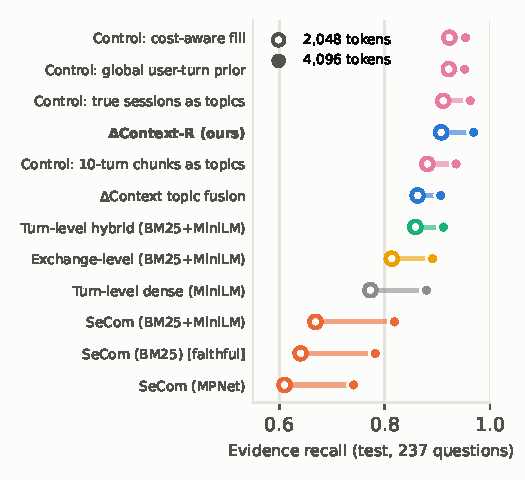
\includegraphics[width=\linewidth]{memory_recall.pdf}
\caption{Evidence recall at 2,048 (open) and 4,096 (filled) context tokens on
237 test questions. Blue: \dc{}; orange: SeCom; pink: topic-free and
grouping controls (Section~\ref{sec:comp}).}
\label{fig:recall}
\end{figure}

\begin{figure}[t]
\centering
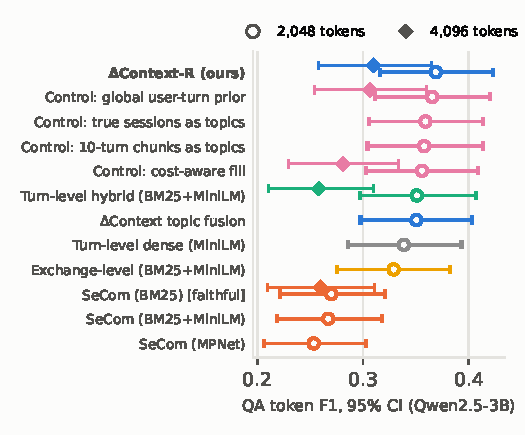
\includegraphics[width=\linewidth]{memory_qa.pdf}
\caption{Answer token F1 with 95\% bootstrap intervals (Qwen2.5-3B reader,
test): circles at 2,048 tokens, diamonds at 4,096 tokens (run for the main
systems). Every system answers worse with the larger budget.}
\label{fig:qa}
\end{figure}

\subsection{Question types}
Fig.~\ref{fig:types} breaks recall down by question type. The largest gains are
on multi-session questions, whose evidence is spread over several sessions
(0.869 vs.\ 0.732 for turn-level hybrid retrieval and 0.387 for SeCom), and on
preference questions (1.000 vs.\ 0.678 and 0.567). Reading the user costs recall
where the evidence is an assistant reply (0.815 vs.\ 0.889 at 2,048 tokens),
the price of the user prior; at 4,096 tokens both reach 1.000.

\begin{figure}[t]
\centering
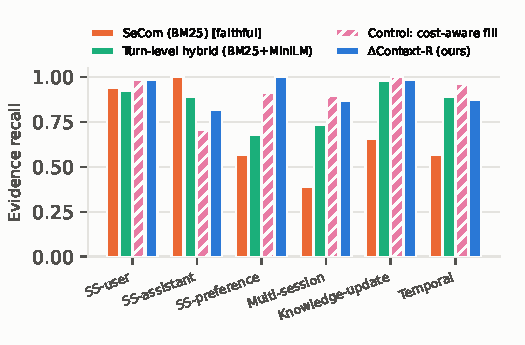
\includegraphics[width=\linewidth]{memory_types.pdf}
\caption{Evidence recall by question type at 2,048 tokens (test).}
\label{fig:types}
\end{figure}

% =====================================================================
\section{Comparisons}
\label{sec:comp}

\subsection{Compared works}
\textbf{SeCom} \cite{pan2025secom} is re-implemented from its code: memory units
are topic segments, keys are their LLMLingua-2 compressions
\cite{pan2024llmlingua2} (xlm-roberta-large, rate 0.75, the turns of a session
compressed jointly), retrieval returns whole units ranked by BM25 (its best
retriever) or MPNet \cite{song2020mpnet}, and units fill the budget in rank
order. SeCom's GPT-4 segmentation needs one API call for each of LongMemEval-S's
19,195 sessions, so we give it \dc{}'s topics cut at session starts, the closest
LLM-free equivalent. We also give it our stronger BM25+MiniLM retriever.
\textbf{LongMemEval's round-level memory} \cite{wu2025longmemeval} is the
exchange-level baseline (a user turn and its replies). \textbf{Turn-level
retrieval} uses dense MiniLM or BM25+MiniLM fusion \cite{cormack2009rrf}, the
strongest baseline here.

\begin{table*}[t]
\centering
\caption{Comparison on 237 LongMemEval-S test questions. Recall: evidence recall; All: share of questions with all evidence retrieved; Turns: mean turns in the 2,048-token context. Differences to \dcr{} in Recall, F1 and EM: $^{***}p<10^{-3}$, $^{*}p<0.05$ (paired bootstrap, Holm); otherwise not significant; --: not run.}
\label{tab:main}
\footnotesize
\setlength{\tabcolsep}{3.0pt}
\begin{tabular}{@{}llccccccccc@{}}
\toprule
& & \multicolumn{4}{c}{2,048 tokens} & \multicolumn{3}{c}{4,096 tokens} & & \\
\cmidrule(lr){3-6}\cmidrule(lr){7-9}
Memory & Unit / keys / retriever & Recall & All & F1 & EM & Recall & All & F1 & Turns & LLM calls \\
\midrule
SeCom \cite{pan2025secom} (faithful) & segment / LLMLingua-2 / BM25 & 0.641$^{***}$ & 0.443 & 0.270$^{***}$ & 0.173$^{*}$ & 0.782$^{***}$ & 0.667 & 0.260 & 11.2 & 1 / session \\
SeCom (MPNet) & segment / LLMLingua-2 / MPNet & 0.610$^{***}$ & 0.426 & 0.253$^{***}$ & 0.160$^{*}$ & 0.741$^{***}$ & 0.608 & -- & 11.6 & 1 / session \\
SeCom (+ our retriever) & segment / LLMLingua-2 / BM25+MiniLM & 0.669$^{***}$ & 0.494 & 0.267$^{***}$ & 0.169$^{*}$ & 0.819$^{***}$ & 0.726 & -- & 11.1 & 1 / session \\
Round-level \cite{wu2025longmemeval} & exchange / raw / BM25+MiniLM & 0.814$^{***}$ & 0.700 & 0.329 & 0.224 & 0.891$^{***}$ & 0.814 & -- & 11.4 & 0 \\
Turn-level dense & turn / raw / MiniLM & 0.773$^{***}$ & 0.658 & 0.339 & 0.232 & 0.880$^{***}$ & 0.797 & -- & 12.6 & 0 \\
Turn-level hybrid & turn / raw / BM25+MiniLM & 0.859 & 0.785 & 0.351 & 0.253 & 0.912$^{***}$ & 0.848 & 0.258$^{*}$ & 11.6 & 0 \\
\dc{} topic fusion & turn+topic / raw / BM25+MiniLM & 0.863 & 0.789 & 0.351 & 0.245 & 0.907$^{***}$ & 0.840 & -- & 11.5 & 0 \\
\textbf{\dcr{} (ours)} & turn+topic / raw / BM25+MiniLM & \textbf{0.908} & \textbf{0.857} & \textbf{0.369} & \textbf{0.253} & \textbf{0.969} & \textbf{0.941} & \textbf{0.310} & 25.3 & \textbf{0} \\
\bottomrule
\end{tabular}
\end{table*}

\subsection{\dcr{} against SeCom}
Against faithful SeCom, \dcr{} improves recall by 0.267 (95\% CI
$[+0.220,+0.314]$) at 2,048 tokens and 0.187 ($[+0.149,+0.228]$) at 4,096, and F1
by 0.099 ($[+0.050,+0.148]$) at 2,048 tokens, all $p<10^{-3}$ (at 4,096 tokens
the F1 gap is $+0.050$, $p{=}0.07$ after correction), while building its memory with no
LLM call and no compression pass (SeCom's LLMLingua-2 pass alone took about two
GPU hours for the 47M tokens of LongMemEval-S, before any segmentation call). Fig.~\ref{fig:grid} shows why
segment-level memory loses here. With every retriever, recall falls as units grow:
turns and exchanges reach 0.66--0.82, topics and sessions only 0.48--0.60,
because a LongMemEval session ($\sim$2.4K tokens) barely fits in the budget and
most of it is assistant text. Finer LLM segments would lie between exchanges and
sessions in size, and even exchanges with the best retriever reach only 0.814 on
test, 0.094 below \dcr{}. LLMLingua-2 denoising does what SeCom reports for dense
retrievers (MPNet on turns: 0.67$\rightarrow$0.75; on topics:
0.48$\rightarrow$0.54), but it does not close the granularity gap.

\begin{figure*}[t]
\centering
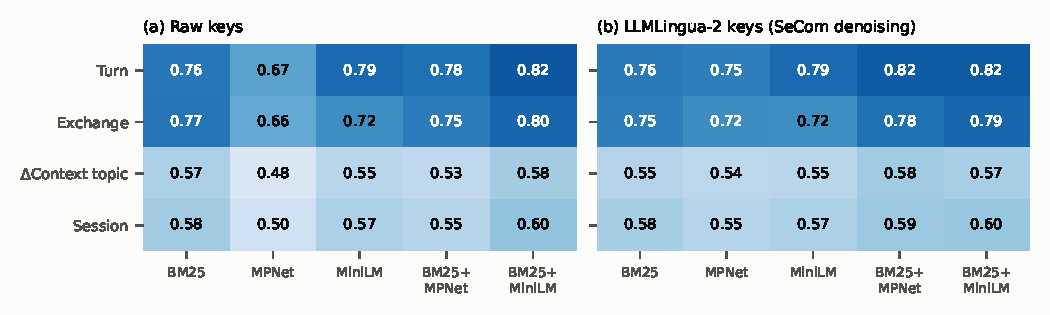
\includegraphics[width=0.85\textwidth]{memory_grid.pdf}
\caption{Dev evidence recall at 2,048 tokens when whole units are retrieved, by
memory unit and retriever, with raw keys (a) and SeCom's LLMLingua-2 keys (b).
Larger units lose with every retriever; compression mainly helps MPNet.}
\label{fig:grid}
\end{figure*}

\subsection{\dcr{} against turn-level retrieval}
Turn-level hybrid retrieval is a much stronger baseline than SeCom on
LongMemEval. \dcr{} beats it by 0.057 recall at 4,096 tokens
($[+0.031,+0.086]$, $p<10^{-3}$) and by 0.049 at 2,048 ($[+0.010,+0.087]$; not
significant after Holm correction). In answers it ties at 2,048 tokens (F1 0.369
vs.\ 0.351, n.s.) and wins at 4,096 (0.310 vs.\ 0.258, $p{=}0.02$). Topic
fusion alone (without reading the user) gives no gain (0.863 vs.\ 0.859).

\subsection{What drives the gain}
Table~\ref{tab:controls} replaces one ingredient at a time, each control tuned on
dev with its own grid. Using true sessions instead of \dc{}'s online topics gives
the same result, and 10-turn chunks are worse (significant at 4,096 tokens), so
the online topics are as good a grouping as the ground truth. Two topic-free
rules, a global bonus for user turns and cost-aware filling (rank score divided
by token cost$^{0.25}$), match \dcr{}: at 2,048 tokens they are 0.014--0.015
higher and at 4,096 0.015--0.017 lower, none significant. The gain therefore comes from
budget-aware reading of user statements; the topic structure contributes on
preference questions (Fig.~\ref{fig:types}), where topic-based variants reach
1.000 against 0.778--0.911 for topic-free rules, but not overall. A diagnostic
on dev explains the design: of the evidence turns that topic fusion misses at
2,048 tokens, 67\% lie inside topics it already read from (78\% for
multi-session questions), so the missing evidence is a user statement that was
ranked low, not an unseen topic. Penalising repeated topics to spread the
budget made recall worse at every strength (0.80--0.60 vs.\ 0.83 on dev).

\begin{table}[t]
\centering
\caption{Ablation on test: recall of \dcr{} minus each control (95\% CI). $^{***}p<10^{-3}$ (Holm); others n.s.}
\label{tab:controls}
\scriptsize
\setlength{\tabcolsep}{2.5pt}
\begin{tabular}{@{}lcc@{}}
\toprule
Control (tuned on dev) & 2,048 tokens & 4,096 tokens \\
\midrule
True sessions as topics & $-$.004 [$-$.029, +.021] & +.007 [$-$.006, +.021] \\
10-turn chunks as topics & +.026 [$-$.005, +.059] & +.033$^{***}$ [+.016, +.054] \\
Global user prior (no topics) & $-$.014 [$-$.050, +.020] & +.017 [$-$.006, +.042] \\
Cost-aware fill (no topics/roles) & $-$.015 [$-$.053, +.023] & +.015 [$-$.008, +.041] \\
Topic fusion (no user reading) & +.045 [+.007, +.082] & +.063$^{***}$ [+.035, +.091] \\
\bottomrule
\end{tabular}
\end{table}

\subsection{Limitations}
Results come from one benchmark, whose sessions are mostly single-topic and
whose evidence is mostly user statements; the user prior helps there and costs
recall where evidence is an assistant reply. The reader is a 3B model scored by
token F1, not an LLM judge, and it answers worse with 4K than with 2K tokens of
context, so recall gains at the larger budget do not all reach the answer.
SeCom's GPT-4 segmentation was replaced by an
LLM-free equivalent, and the exchange-level baseline bounds what finer segments
could reach. Dev selection over many configurations made dev gains optimistic,
which is why every claim above rests on the single test pass.

% =====================================================================
\section{Conclusion}
\label{sec:concl}
This paper presented \dcr{}, a conversational memory that stores a growing chat
as topics found online, with no language model, and retrieves by reading the
user's statements inside the most relevant topics under a fixed token budget.
Against segment-level memory with compression-based denoising, it raised
evidence recall from 0.64 to 0.91 and answer F1 by 37\% at the same budget and
reader, and at the larger budget it beat strong turn-level hybrid retrieval.
Its novelty is a retrieval rule shaped by the budget: rank turns with lexical,
dense and topic evidence, then spend the budget on short user statements in the
topics already judged relevant. Controlled ablations showed that this
budget-aware reading, rather than topic structure itself, drives the gain,
while the online topics proved as good a grouping as the true sessions. Future
work will test the rule on benchmarks whose sessions mix several topics, and
learn the user prior and budget split from the question instead of fixing them.

% =====================================================================
\begin{thebibliography}{99}

\bibitem{ni2023survey}
J.~Ni, T.~Young, V.~Pandelea, F.~Xue, and E.~Cambria, ``Recent advances in deep learning based dialogue systems: A systematic survey,'' \emph{Artificial Intelligence Review}, vol.~56, no.~4, pp.~3055--3155, 2023, doi: 10.1007/s10462-022-10248-8.

\bibitem{wang2024agents}
L.~Wang, C.~Ma, X.~Feng, Z.~Zhang, H.~Yang, J.~Zhang, Z.~Chen, J.~Tang, X.~Chen, Y.~Lin, W.~X. Zhao, and Z.~Wei, ``A survey on large language model based autonomous agents,'' \emph{Frontiers of Computer Science}, vol.~18, no.~6, Art.~no.~186345, 2024, doi: 10.1007/s11704-024-40231-1.

\bibitem{zhang2025memory}
Z.~Zhang, Q.~Dai, X.~Bo, C.~Ma, R.~Li, X.~Chen, J.~Zhu, Z.~Dong, and J.-R. Wen, ``A survey on the memory mechanism of large language model-based agents,'' \emph{ACM Transactions on Information Systems}, vol.~43, no.~6, pp.~1--47, 2025, doi: 10.1145/3748302.

\bibitem{tay2022efficient}
Y.~Tay, M.~Dehghani, D.~Bahri, and D.~Metzler, ``Efficient transformers: A survey,'' \emph{ACM Computing Surveys}, vol.~55, no.~6, pp.~1--28, 2022, doi: 10.1145/3530811.

\bibitem{liu2024lost}
N.~F. Liu, K.~Lin, J.~Hewitt, A.~Paranjape, M.~Bevilacqua, F.~Petroni, and P.~Liang, ``Lost in the middle: How language models use long contexts,'' \emph{Transactions of the Association for Computational Linguistics}, vol.~12, pp.~157--173, 2024, doi: 10.1162/tacl\_a\_00638.

\bibitem{huang2025hallucination}
L.~Huang, W.~Yu, W.~Ma, W.~Zhong, Z.~Feng, H.~Wang, Q.~Chen, W.~Peng, X.~Feng, B.~Qin, and T.~Liu, ``A survey on hallucination in large language models: Principles, taxonomy, challenges, and open questions,'' \emph{ACM Transactions on Information Systems}, vol.~43, no.~2, pp.~1--55, 2025, doi: 10.1145/3703155.

\bibitem{wu2026rag}
S.~Wu, Y.~Xiong, Y.~Cui, H.~Wu, C.~Chen, Y.~Yuan, L.~Huang, X.~Liu, T.-W. Kuo, N.~Guan, and C.~J. Xue, ``Retrieval-augmented generation for natural language processing: A survey,'' \emph{Artificial Intelligence Review}, vol.~59, no.~9, Art.~no.~192, 2026, doi: 10.1007/s10462-026-11605-7.

\bibitem{zhao2024dense}
W.~X. Zhao, J.~Liu, R.~Ren, and J.-R. Wen, ``Dense text retrieval based on pretrained language models: A survey,'' \emph{ACM Transactions on Information Systems}, vol.~42, no.~4, pp.~1--60, 2024, doi: 10.1145/3637870.

\bibitem{pan2024vectordb}
J.~J. Pan, J.~Wang, and G.~Li, ``Survey of vector database management systems,'' \emph{The VLDB Journal}, vol.~33, no.~5, pp.~1591--1615, 2024, doi: 10.1007/s00778-024-00864-x.

\bibitem{wang2025recursive}
Q.~Wang, Y.~Fu, Y.~Cao, S.~Wang, Z.~Tian, and L.~Ding, ``Recursively summarizing enables long-term dialogue memory in large language models,'' \emph{Neurocomputing}, vol.~639, Art.~no.~130193, 2025, doi: 10.1016/j.neucom.2025.130193.

\bibitem{zhong2024memorybank}
W.~Zhong, L.~Guo, Q.~Gao, H.~Ye, and Y.~Wang, ``MemoryBank: Enhancing large language models with long-term memory,'' in \emph{Proc. AAAI Conf. Artificial Intelligence}, vol.~38, no.~17, pp.~19724--19731, 2024, doi: 10.1609/aaai.v38i17.29946.

\bibitem{packer2023memgpt}
C.~Packer, S.~Wooders, K.~Lin, V.~Fang, S.~G. Patil, I.~Stoica, and J.~E. Gonzalez, ``MemGPT: Towards LLMs as operating systems,'' arXiv:2310.08560, 2023.

\bibitem{wu2025longmemeval}
D.~Wu, H.~Wang, W.~Yu, Y.~Zhang, K.-W. Chang, and D.~Yu, ``LongMemEval: Benchmarking chat assistants on long-term interactive memory,'' in \emph{Proc. Int. Conf. Learning Representations (ICLR)}, 2025.

\bibitem{pan2025secom}
Z.~Pan, Q.~Wu, H.~Jiang, X.~Luo, H.~Cheng, D.~Li, Y.~Yang, C.-Y. Lin, H.~V. Zhao, L.~Qiu, and J.~Gao, ``On memory construction and retrieval for personalized conversational agents,'' in \emph{Proc. Int. Conf. Learning Representations (ICLR)}, 2025.

\bibitem{pan2024llmlingua2}
Z.~Pan, Q.~Wu, H.~Jiang, M.~Xia, X.~Luo, J.~Zhang, Q.~Lin, V.~R{\"u}hle, Y.~Yang, C.-Y. Lin, H.~V. Zhao, and L.~Qiu, ``LLMLingua-2: Data distillation for efficient and faithful task-agnostic prompt compression,'' in \emph{Findings of the Association for Computational Linguistics: ACL 2024}, 2024, pp.~963--981, doi: 10.18653/v1/2024.findings-acl.57.

\bibitem{ma2024topicaware}
X.~Ma, Y.~Xu, H.~Zhao, and Z.~Zhang, ``Multi-turn dialogue comprehension from a topic-aware perspective,'' \emph{Neurocomputing}, vol.~578, Art.~no.~127385, 2024, doi: 10.1016/j.neucom.2024.127385.

\bibitem{xu2025umlf}
J.~Xu, F.~Jiang, A.~Gao, L.~F. D'Haro, and H.~Li, ``Unsupervised mutual learning of discourse parsing and topic segmentation in dialogue,'' \emph{IEEE Transactions on Audio, Speech and Language Processing}, vol.~33, pp.~4667--4681, 2025, doi: 10.1109/TASLPRO.2025.3623884.

\bibitem{lavarec2026chunking}
E.~Lavarec and Y.~Du, ``Evaluating document chunking approaches for retrieval augmented generation in editorial content,'' \emph{IAES International Journal of Artificial Intelligence}, vol.~15, no.~2, pp.~1909--1918, 2026, doi: 10.11591/ijai.v15.i2.pp1909-1918.

\bibitem{hearst1997texttiling}
M.~A. Hearst, ``TextTiling: Segmenting text into multi-paragraph subtopic passages,'' \emph{Computational Linguistics}, vol.~23, no.~1, pp.~33--64, 1997.

\bibitem{xing2021csm}
L.~Xing and G.~Carenini, ``Improving unsupervised dialogue topic segmentation with utterance-pair coherence scoring,'' in \emph{Proc. 22nd Annu. Meeting Special Interest Group on Discourse and Dialogue (SIGDIAL)}, 2021, pp.~167--177, doi: 10.18653/v1/2021.sigdial-1.18.

\bibitem{gao2023dialstart}
H.~Gao, R.~Wang, T.-E. Lin, Y.~Wu, M.~Yang, F.~Huang, and Y.~Li, ``Unsupervised dialogue topic segmentation with topic-aware contrastive learning,'' in \emph{Proc. 46th Int. ACM SIGIR Conf. Research and Development in Information Retrieval}, 2023, pp.~2481--2485, doi: 10.1145/3539618.3592081.

\bibitem{jiang2023superdialseg}
J.~Jiang, C.~Dong, S.~Kurohashi, and A.~Aizawa, ``SuperDialseg: A large-scale dataset for supervised dialogue segmentation,'' in \emph{Proc. Conf. Empirical Methods in Natural Language Processing (EMNLP)}, 2023, pp.~4086--4101, doi: 10.18653/v1/2023.emnlp-main.249.

\bibitem{langchain2024semantic}
LangChain, ``SemanticChunker (langchain\_experimental.text\_splitter),'' 2024. [Online]. Available: \url{https://python.langchain.com}

\bibitem{robertson2009bm25}
S.~Robertson and H.~Zaragoza, ``The probabilistic relevance framework: BM25 and beyond,'' \emph{Foundations and Trends in Information Retrieval}, 2009, doi: 10.1561/1500000019.

\bibitem{reimers2019sbert}
N.~Reimers and I.~Gurevych, ``Sentence-BERT: Sentence embeddings using Siamese BERT-networks,'' in \emph{Proc. Conf. Empirical Methods in Natural Language Processing and Int. Joint Conf. Natural Language Processing (EMNLP-IJCNLP)}, 2019, pp.~3980--3990, doi: 10.18653/v1/D19-1410.

\bibitem{song2020mpnet}
K.~Song, X.~Tan, T.~Qin, J.~Lu, and T.-Y. Liu, ``MPNet: Masked and permuted pre-training for language understanding,'' in \emph{Advances in Neural Information Processing Systems (NeurIPS)}, 2020.

\bibitem{cormack2009rrf}
G.~V. Cormack, C.~L.~A. Clarke, and S.~Buettcher, ``Reciprocal rank fusion outperforms Condorcet and individual rank learning methods,'' in \emph{Proc. 32nd Int. ACM SIGIR Conf. Research and Development in Information Retrieval}, 2009, pp.~758--759, doi: 10.1145/1571941.1572114.

\bibitem{veena2023agroner}
G.~Veena, V.~Kanjirangat, and D.~Gupta, ``AGRONER: An unsupervised agriculture named entity recognition using weighted distributional semantic model,'' \emph{Expert Systems with Applications}, vol.~229, Art.~no.~120440, 2023, doi: 10.1016/j.eswa.2023.120440.

\bibitem{veena2023relation}
G.~Veena, D.~Gupta, and V.~Kanjirangat, ``Semi-supervised bootstrapped syntax-semantics-based approach for agriculture relation extraction for knowledge graph creation and reasoning,'' \emph{IEEE Access}, vol.~11, pp.~138375--138398, 2023, doi: 10.1109/ACCESS.2023.3339552.

\bibitem{venugopalan2022guidedlda}
M.~Venugopalan and D.~Gupta, ``An enhanced guided LDA model augmented with BERT based semantic strength for aspect term extraction in sentiment analysis,'' \emph{Knowledge-Based Systems}, vol.~246, Art.~no.~108668, 2022, doi: 10.1016/j.knosys.2022.108668.

\bibitem{gurusamy2023summarization}
B.~M. Gurusamy, P.~K. Rengarajan, and P.~Srinivasan, ``A hybrid approach for text summarization using semantic latent Dirichlet allocation and sentence concept mapping with transformer,'' \emph{International Journal of Electrical and Computer Engineering}, vol.~13, no.~6, pp.~6663--6672, 2023, doi: 10.11591/ijece.v13i6.pp6663-6672.

\bibitem{qwen2024qwen25}
Qwen Team, ``Qwen2.5 technical report,'' arXiv:2412.15115, 2024.

\bibitem{holm1979simple}
S.~Holm, ``A simple sequentially rejective multiple test procedure,'' \emph{Scandinavian Journal of Statistics}, vol.~6, no.~2, pp.~65--70, 1979.

\bibitem{xie2021tiage}
H.~Xie, Z.~Liu, C.~Xiong, Z.~Liu, and A.~Copestake, ``TIAGE: A benchmark for topic-shift aware dialog modeling,'' in \emph{Findings of the Association for Computational Linguistics: EMNLP 2021}, 2021, pp.~1684--1690, doi: 10.18653/v1/2021.findings-emnlp.145.

\bibitem{xu2021dialseg711}
Y.~Xu, H.~Zhao, and Z.~Zhang, ``Topic-aware multi-turn dialogue modeling,'' in \emph{Proc. AAAI Conf. Artificial Intelligence}, vol.~35, no.~16, pp.~14176--14184, 2021, doi: 10.1609/aaai.v35i16.17668.

\end{thebibliography}

\end{document}
